\section{\piz Production} \label{sec:into:xsection}
The present analysis uses two approaches to describe the behavior of the \piz cross-section. One approach is for incident photon beam energies less than 2.8~GeV where the missing resonance search is most valid and the data can be described well by coupling of the \piz electromagnetic wave functions. The second approach attempts to describe the behavior of the \piz by using General Parton Distribution models, \abbr{GPD} for incident photon beam energies greater than 2.8~GeV.
%The physics behind this is that since the photon couples to charged-fermion pairs, a part of its cross-section could be described by considering interactions between the hadron and a virtual fermion pair~\cite{butterworth}.


\subsection{Low Energy \piz Production}\label{sec:into:xsection.low}

\begin{figure}[h!]\begin{center}
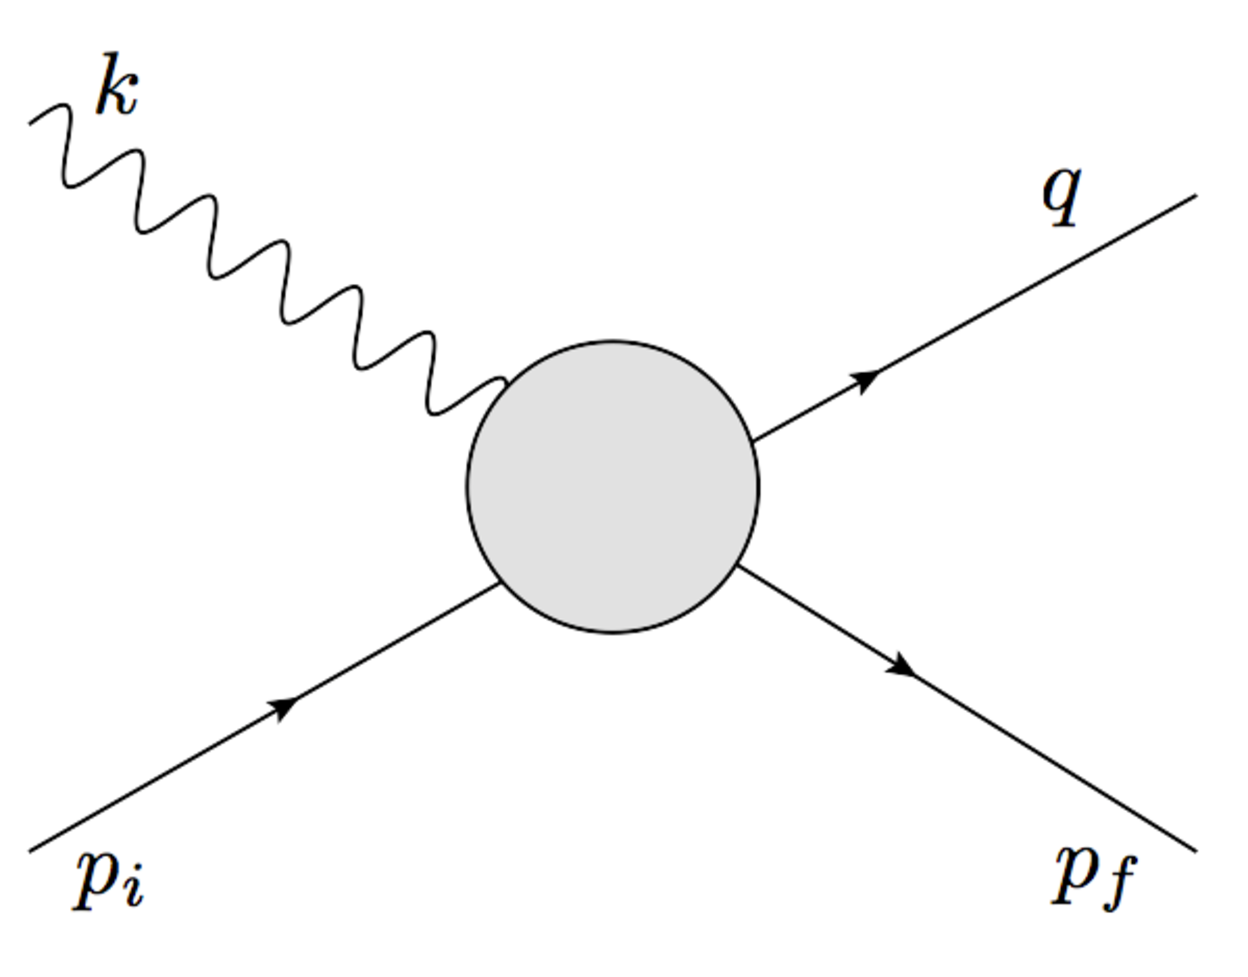
\includegraphics[width=0.5 \figwidth,height= \qfigheight]{\figures/feyman_pi0IV.pdf}
\caption[Diagram for photoproduction of the \piz meson]{\label{fig:xsection.pi0feynman}	Diagram for photoproduction of the \piz meson. $k$ and $p_i$ are the incident photon beam and target proton 4-moment respectively, $q$ and $p_f$ represent the produced \piz meson and scattered proton 4-momenta respectively.}
\end{center}\end{figure}
For incoming photon beam energies less than 2.8~GeV, the production of the \piz meson, with 4-momenta $q$, in photon-proton reactions, with 4-momenta $k$ and $p_i$ respectively and $p_f$ being the 4-momenta of the scattered proton (see Fig.~\ref{fig:xsection.pi0feynman}),  can be described in terms of the three Lorentz invariant Mandelstam variables, $s$, $t$ and $u$, where
\begin{align}
s = (k+p_i)^2 = (q+p_f)^2 \nonumber \\
t=(p_i-p_f)^2 = (k-q)^2  \nonumber \\
u = (k - p_f)^2 = (p_i-q)^2 \ .
\end{align}
The sum of the Mandelstam variables linearly combine to give the sum of masses of the particles involved:
\begin{align}
s + t + u = \sum\limits_{i}^{4} m_i^2 
\end{align}
and the definition of Lorentz-invariant mass:
\begin{align}
p_i\cdot p_i = E_i^2 - \mathbf{p_i}\cdot \mathbf{p_i} = m_i^2 \ .
\end{align}
Using energy-momentum conservation:
\begin{align}
k + p_i = q+p_f \,
\end{align}
it is seen that only three of the four momenta are independent. Conventionally the use of $k$ and $q$ and a combined 4-momenta of the nuclei 
\begin{align}
P = \frac{1}{2}(p_i+p_f)
\end{align}
are used as the independent kinematic variables. The three Mandelstam variables can be express in terms of the other two, therefore the scattering process is described by functions of only two of the Mandelstam variables. Conventionally they are chosen to be $s$ and $t$, which in the center-of-mass frame (C.M.) of the initial and final state equal the invariant mass squared of the system and the momentum transfer in the production process respectively.
\subsection{Isospin Representation}\label{sec:isospin}
The scattering matrix $\mathcal{M}$ for single pion photoproduction process is written as:
\begin{align}
\mathcal{M} =  (\epsilon_\mu k_\nu - \epsilon_\nu k_\mu)&[ \frac{1}{2}i \gamma_5 \gamma_\mu \gamma_\nu A_1(s,t) + 2 i \gamma_5 P_\mu(q-\frac{1}{2}k)_\nu A_2(s,t) \nonumber \\ & + \gamma_5 \gamma_\mu q_\nu A_3(s,t) + \gamma_5 \gamma_\mu(2P_\nu- i M\gamma_\nu) A_4(s,t) ] \ ,
\end{align}
where $M$ is the nucleon mass, $\epsilon$ is the photon polarization and $A_i(s,t)$ are the invariant functions of the Mandelstam invariants $s$ and $t$. The amplitude $A_i(s,t)$ refers to the emission of a pion of isospin index $\alpha$, and is given by the well-known formula:
\begin{align}\label{eq:isoscal_vec}
A_i(s,t)= A_i^{(0)}\tau_\alpha + A_i^{(+)}\delta_{\alpha 0} + \frac{1}{2} A_i^{(-)}\left[\tau_\alpha,\tau_0\right] \ ,
\end{align}
where $\tau_\alpha$ are the nucleon isospin transition operators, where the sign of $\alpha$ indicates the opposite sign of the pion isospin, this is by convention. Eq.~\ref{eq:isoscal_vec} assumes that the photon interaction with hadrons occurs through isoscalar and isovector parts, so that $A_i^{(0)}$ is the isoscalar amplitude that corresponds to a zero net isospin transistion resulting from the electromagnetic field. The amplitudes $A_i^{(+)}$ and $A_i^{(-)}$ are the isovector amplitudes and can be combined as $A_i^{(+)} + 2 A_i^{(-)}$ and $A_i^{(+)} - A_i^{(-)}$ so that the pion nucleon final state has definite isospin $\frac{1}{2}$ and $\frac{3}{2}$ respectively~\cite{Rosenfeld} by use of
\begin{align}
A^S = -(3)^\frac{1}{2}A^{(0)} \nonumber \\
A^{V1} = \left(\frac{1}{3}\right)^\frac{1}{2}A_i^{(+)} + 2 A_i^{(-)} \nonumber \\
A^{V2} = \left(\frac{2}{3}\right)^\frac{1}{2}A_i^{(+)} - A_i^{(-)} \ ,
\end{align}
where $A^S$, $A^{V1}$ and $A^{V2}$ are the isoscalar amplitude, isovector amplitude of isospin $\frac{1}{2}$ and isovector amplitude of isospin $\frac{3}{2}$ respectively.
The four possible pion nucleon amplitudes $A_i(s,t)$ of the initial and final state particles in the pion photoproduction process are in terms of the isoscalar and isovector are:
\begin{align}
A_1(\gamma p \to n \pi^+) = -\sqrt{\frac{1}{3}}A^{V3} + \sqrt{\frac{2}{3}}(A^{V1} - A^{S}),\\
A_2(\gamma p \to p \pi^0) = \sqrt{\frac{2}{3}} A^{V3} + \sqrt{\frac{1}{3}}(A^{V1}-A^{S}),\\
A_3(\gamma n \to p \pi^-) = \sqrt{\frac{1}{3}}A^{V3} - \sqrt{\frac{2}{3}}(A^{V1} + A^{S}),\\
A_3(\gamma n \to n \pi^0) = \sqrt{\frac{2}{3}}A^{V3} + \sqrt{\frac{1}{3}}(A^{V1} + A^{S}).
\end{align}
Since the combination $\sqrt{\frac{2}{3}}(A^{V1} \mp A^{S})$ gives the coupling of photons to positive and neutral isospin-$\frac{1}{2}$ states, respectively, ~\protect\cite{Rosenfeld}, defined explicitly
%
\begin{align}
&&A^p = + \sqrt{\frac{2}{3}}(A^{V1} - A^{S}),\\
&&A^n = -\sqrt{\frac{2}{3}}(A^{V1} + A^{S}).
\end{align}
\subsection{Structure Functions}\label{sec:CGLN}
To obtain the scattering matrix elements in terms of experimental quantities, it is preferred and easier to work in the C.M. system and reduce the $\mathcal{M}$ to a form $\mathcal{F}$ by equating the invariant form of the scattering matrix elements in each frame, i.e.:
\begin{align}
\bar{u}(p_2)\mathcal{M} u(p_1) \equiv \frac{4 \pi W}{M}\chi_f^\dagger \mathcal{F} \chi_i \ ,
\end{align}
where $\bar{u}(p_2)$ and $u(p_1)$ are final and initial state Dirac spinors respectively and $\chi_f$ and $\chi_i$ are final and initial state Pauli spinors. The differential cross-section for single pion production is:
\begin{align}
\frac{d\sigma}{d\Omega} = \frac{q}{k}| \bra{f}\mathcal F \ket{i}|^2,
\end{align}
The expression to express Dirac spinors in terms of Pauli spinors is written as:
\begin{align}
\mathcal{F} = & i\vec{\mathbf{\sigma}}\cdot \vec{\mathbf{\epsilon}} \mathcal{F}_1 + \frac{1}{qk}(\vec{\mathbf{\sigma}}\cdot \vec{\mathbf{q}})\vec{\mathbf{\sigma}} \cdot(\vec{\mathbf{k}}\times \vec{\mathbf{\epsilon}}) \mathcal{F}_2 \nonumber \\ & + \frac{i}{qk}(\vec{\mathbf{\sigma}}\cdot \vec{\mathbf{k}})(\vec{\mathbf{q}}\cdot \vec{\mathbf{\epsilon}})\mathcal{F}_3 + \frac{i}{q^2}(\vec{\mathbf{\sigma}}\cdot \vec{\mathbf{q}})(\vec{\mathbf{q}}\cdot \vec{\mathbf{\epsilon}})\mathcal{F}_4 \ ,
\end{align}
where $\vec{\mathbf{k}}$ and $\vec{\mathbf{q}}$ are the C.M. 3-momenta and $\vec{\mathbf{\epsilon}}$ is the polarization of the photon. The relationship between $A_i$ and $\mathcal{F}$ is found using the relations:
\begin{align}
\mathcal{F}_1 = \frac{W- M}{8 \pi W }(D_1 D_2)^{\frac{1}{2}}\left[ A_1+(W-M)A_4 - \frac{k_0q_0-\vec{\mathbf{k}}\cdot \vec{\mathbf{q}}}{W-M}(A_3-A_4)\right] \\
\mathcal{F}_2 = qk \frac{W- M}{8 \pi W }(\frac{D_2}{D_1})^{\frac{1}{2}}\left[ -A_1+(W+M)A_4 + \frac{k_0q_0-\vec{\mathbf{k}}\cdot \vec{\mathbf{q}}}{W+M}(A_3-A_4)\right]  \\
\mathcal{F}_3 =qk \frac{W- M}{8 \pi W }(D_1 D_2)^{\frac{1}{2}}q\left[(W-M)A_2 + A_3 - A_4\right]\\
\mathcal{F}_4 = q^2 \frac{W- M}{8 \pi W }(\frac{D_2}{D_1})^{\frac{1}{2}}q\left[ -(W+M)A_2 + A_3 - A_4\right] 
\end{align}
where
\begin{align}
D_1 = (M^2 + \vec{\mathbf{k}}^2)^{\frac{1}{2}}+M \\
D_2 = (M^2 + \vec{\mathbf{q}}^2)^{\frac{1}{2}}+M \ .
\end{align}
$\mathcal{F}_i(s,t)$ are known as structure functions, alternatively known by Chew, Goldberger, Low and Nambu (\abbr{CGLN}) amplitudes. These amplitudes describe photoproduction as a function of $s$ and $t$, and therefore in terms of momentum transfer. To represent the process in terms of angular momentum transitions, expansion of the structure functions as partial waves in derivatives of Legendre polynomials, $P_l^\prime(\cos\theta)$, results in the four multipole series:
\begin{align}
&&\mathcal{F_1} = \displaystyle\sum_{l=0}^{\infty}[lM_{l+} + E_{l^+}]P_{l+1}^{\prime}(\cos\theta) + [(l+1)M_{l-1} + E_{l-}]P_{l-1}^{\prime}(\cos\theta)\\
&&\mathcal{F_2} = \displaystyle\sum_{l=1}^{\infty}[(l+1)M_{l+}+lM_{l-}]P_{l}^{\prime}(\cos\theta)\\
&&\mathcal{F_3} = \displaystyle\sum_{l=1}^{\infty}[E_{l+}-M_{l+}]P_{l+1}^{\prime \prime}(\cos\theta) + [E_{l-} + M_{l-}]P_{l-1}^{\prime \prime}(\cos\theta)\\
&&\mathcal{F_4} = \displaystyle\sum_{l=1}^{\infty}[M_{l+} - E_{l+} - M_{l-} - E_{l-}]P_{l}^{\prime \prime}(\cos\theta)
\end{align}
The energy-dependent amplitudes $M_{l\pm}$ and $E_{l\pm}$ refer to transitions initiated by magnetic and electric radiation, respectively, leading to final states of orbital angular momentum $l$ and total angular momentum $j=l\pm\frac{1}{2}$. 

The energy-dependent amplitudes $M_{l\pm}$ and $E_{l\pm}$ cannot be extracted directly from measurements, however using models on measured differential cross-sections and polarizations aide in the determination of the amplitudes. Constraining the production amplitudes aides in the determination of resonances. One such model that is used in this thesis is the SAID parameterization model discussed in Sec~\ref{sec:intro.said}. 


\subsection{SAID}\label{sec:intro.said}

SAID~\cite{SAID} is a repository of experimental data and an interactive analysis facility, allowing to compare and extract data and partial wave solutions (PWA) for a variety of photoproduction, electro-production and pion production reactions. It was created by R. A. Arndt and L. D. Roper for the use of verifying model calculations against measured/fitted data, compare model calculations against SAID predictions for unmeasured observables, experimental planning, and simulations and event generators.

SAID is based upon the theoretical framework given in~\ref{sec:isospin}. SAID generates resonance couplings, in terms of angular momentum and isospin quantum numbers, that are extracted from a fit-based determination of multipoles using both an energy-dependent and an energy-independent parametrization. The photoproduction amplitude is assumed to be in the form of a Breit-Wigner and a background term in the form of~\cite{ar90};
\begin{align}
A=A_l(1+iT_\pi)=A_r\left(\frac{k_0q_0}{kq}\right)^{\frac{1}{2}} \frac{W_0\sqrt{\Gamma \Gamma_{\gamma}}}{W_0^2-W^2-iW_0\Gamma} \ ,
\end{align}
in which $A_l$ is the background parameter, $W_0$, $\Gamma$ and $\Gamma_{\gamma}$ are functions of the full width $\Gamma_{0}$ and $A_R$ being the resonant parameter in the form of;
\begin{align}
A_r=\frac{\mu}{q}\left(\frac{k}{q}\right)^l\sum_{n=0}^{N}p_n\left(\frac{E_{\pi}}{\mu}\right)^n
\end{align}
where $k_0$ and $q_0$ are the pion and photon momenta at the resonance energy, $\mu$ is the pion mass, $E_{\pi}$ is the pion kinetic energy in the lab frame and $p_n$ is a free parameter. The background term is expanded as a set of Legendre polynomial terms with associated free parameters along with a sum of a pseudoscalar Born partial waves, which are determined by fitting the data. Multipoles can then be extracted by a fit of $A$ close to the resonance position.

\subsection{Summary}
A full set of differential cross-sections and polarization observables is required for the determination of multipoles. These can be related to the invariant amplitudes as functions of $W$ and $\cos\theta$. For the separation of the different isospin contributions, both the proton and the neutron pion-photoproduction measurements are needed. An understanding of the invariant amplitudes, and subsequent CGLN structure functions, can provide information on the multipole transitions taking place. This  allows to get direct information about the quantum numbers of the produced resonant states and constrain their position, widths and couplings.
The work of this thesis is devoted to measuring of the differential cross-sections for better fit determinations and possible resonance searches using the SAID parameterizations.
\subsection{High Energy \piz Production}\label{sec:into:xsection.high}
%ere is the citation ~\cite{key1, key2,Rad1996, Diehl}
The production of the \piz meson in photon-proton reactions, for incoming photon beam energies greater than 2.8~GeV, is considered to be a hard exclusive reaction. One approach to study the \piz production, in photon-proton reactions, is use the handbag model. In the handbag approach, the reaction is factorized into two parts. The first part is when one quark from the incoming and one from the outgoing nucleon participate in the hard sub-process, small blob in Fig.~\ref{fig:xsection.handbag}. This hard sub-process is achieved when the incident photon excites a quark, since quarks are bound quantum particles, the excited quark produces a jet of quarks that form the meson and then de-excites back into the nucleon. This is calculable using pQCD. The second part ,the soft part seen as the large blob in Fig.~\ref{fig:xsection.handbag} , consists of all the other quarks that are spectators and can be described in terms of GPDs~\cite{key1, key2,Rad1996, Diehl}. The hard exclusive meson (M) photo-production process factorizes into, $\gamma q \to Mq$, this is depicted in Fig.~\ref{fig:xsection.handbag}. The handbag mechanism is applicable when the Mandelstam variables, $s$, $t$, $u$, are large as compared to a hadronic scale of order 1 GeV . In Ref.~\cite{Huang2000} a model, derived from the handbag approach, has been applied to predict angular dependence of scaled photoproduction cross section of \piz and is illustrated in Fig.~\ref{fig:xsection.handbag.cal}. In the analysis presented, this model will investigated using the data obtained in \abbr{CLAS}.

\begin{figure}[h!]\begin{center}
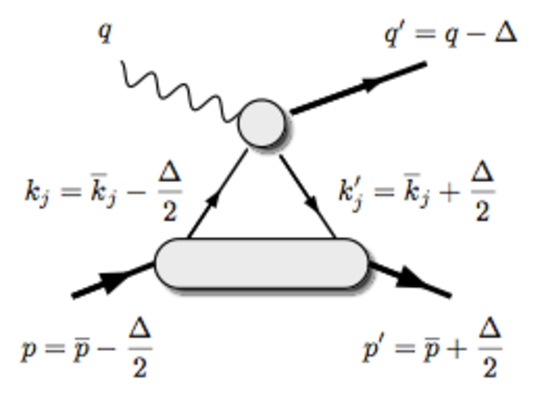
\includegraphics[width= 0.8 \figwidth ,height=\qfigheight]{\grpath/intro/handbag.pdf}
\caption[The handbag-type diagram for photoproduction of mesons]{\label{fig:xsection.handbag}	The handbag-type diagram for photoproduction of mesons. The large blob represents a sum over all spectator configuration. $k_j$ and $k_j^{\prime}$  denote the momenta of the active partons. The small blob stands for meson photoproduction off partons.}
\end{center}\end{figure}

\begin{figure}[h!]\begin{center}
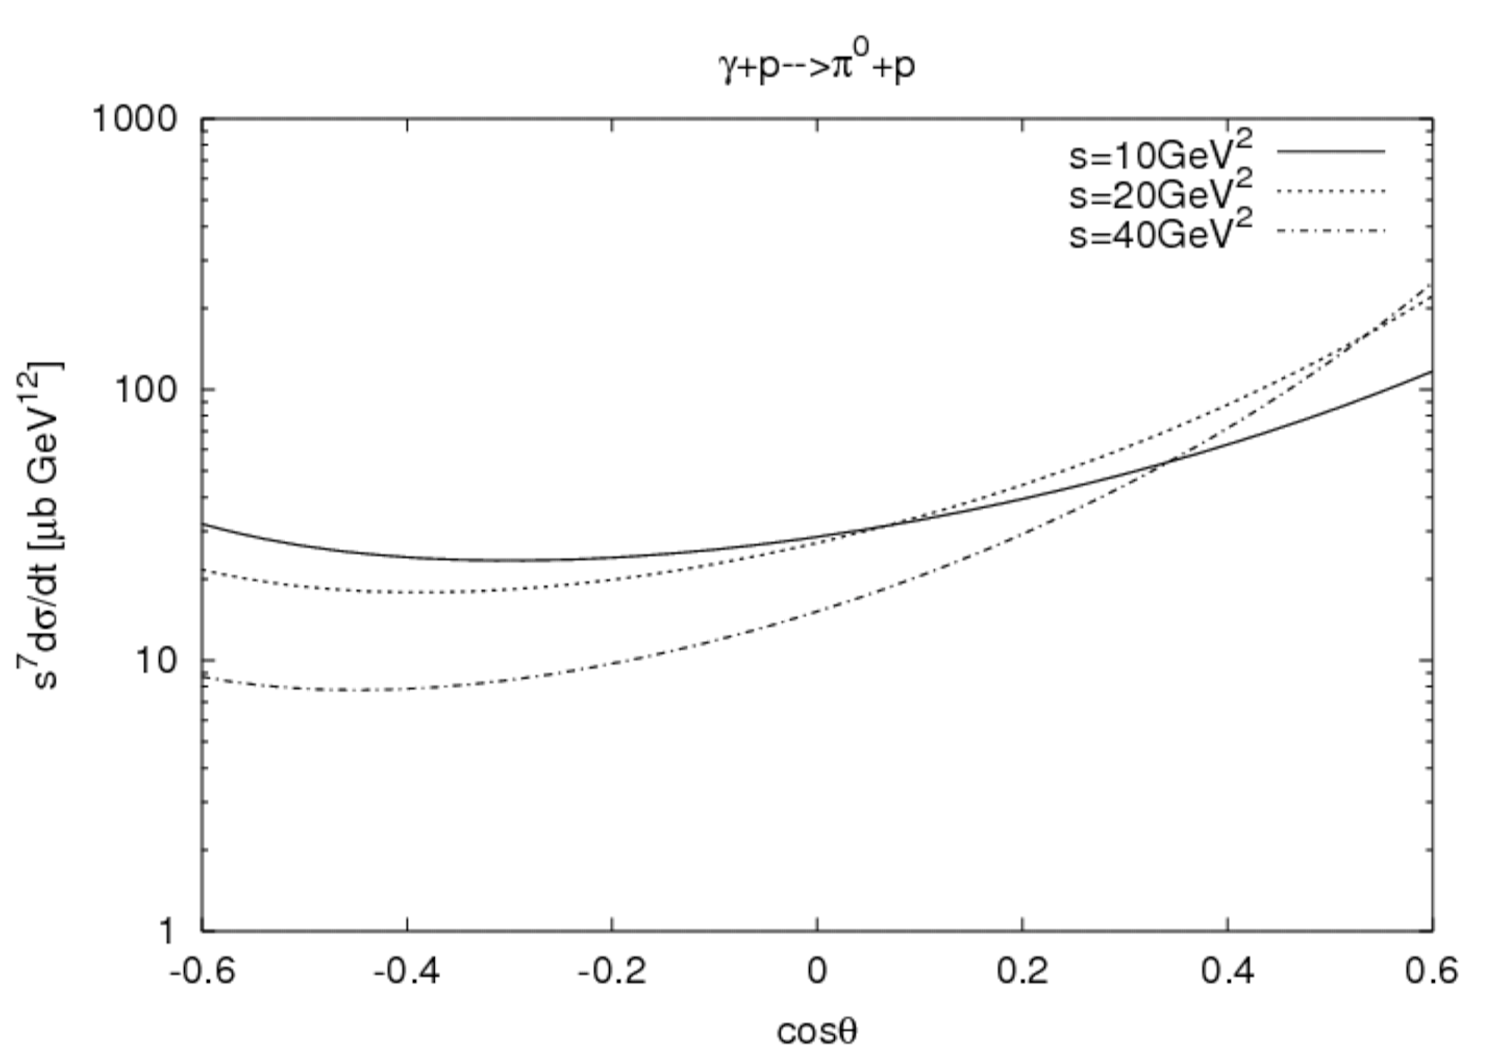
\includegraphics[width= 0.8 \figwidth ,height=\qfigheight]{\grpath/intro/photo-fig7.pdf}
\caption[The soft physics contribution to the cross-section for photoproduction of \piz]{\label{fig:xsection.handbag.cal}The soft physics contribution to the cross-section for photoproduction of \piz scaled by s$^7$ versus $\cos\theta$, where $\theta$ is the scattering angle in the $\gamma p$ c.m. system~\cite{Huang2000}.}
\end{center}\end{figure}
\FloatBarrier


% %